%% This is the ctufit-thesis example file. It is used to produce theses
%% for submission to Czech Technical University, Faculty of Information Technology.
%%
%% This is version 1.4.2, built 20. 3. 2025.
%% 
%% Get the newest version from
%% https://gitlab.fit.cvut.cz/theses-templates/FITthesis-LaTeX
%%
%%
%% Copyright 2024, Tomas Novacek
%% Copyright 2021, Eliska Sestakova and Ondrej Guth
%%
%% This work may be distributed and/or modified under the
%% conditions of the LaTeX Project Public License, either version 1.3
%% of this license or (at your option) any later version.
%% The latest version of this license is in
%%  https://www.latex-project.org/lppl.txt
%% and version 1.3 or later is part of all distributions of LaTeX
%% version 2005/12/01 or later.
%%
%% This work has the LPPL maintenance status `maintained'.
%%
%% The current maintainer of this work is Tomas Novacek (novacto3@fit.cvut.cz).
%% Alternatively, submit bug reports to the tracker at
%% https://gitlab.fit.cvut.cz/theses-templates/FITthesis-LaTeX/issues
%%
%%

% arara: xelatex
% arara: biber
% arara: xelatex
% arara: xelatex

%%%%%%%%%%%%%%%%%%%%%%%%%%%%%%%%%%%%%%%%%
% CLASS OPTIONS
% language: czech/english/slovak
% thesis type: bachelor/master/dissertation
% colour: bw for black&white OR no option for default colour scheme
% electronic (oneside) or printed (twoside), twoside is default
% paragraph - if passed, this optional argument sets paragraphs as the deepest level of headers, styles it, numbers it and adds it to Table of Content. Use with care! Normally, it is considered unwise to use it, since its too deep.
%%%%%%%%%%%%%%%%%%%%%%%%%%%%%%%%%%%%%%%%%
\documentclass[english,bachelor,oneside]{ctufit-thesis}

%%%%%%%%%%%%%%%%%%%%%%%%%%%%%%%%%%
% FILL IN THIS INFORMATION
%%%%%%%%%%%%%%%%%%%%%%%%%%%%%%%%%%
\ctufittitle{Mutation testing for the R language} % replace with the title of your thesis
\ctufitauthorfull{Assanali Amandykov} % replace with your full name (first name(s) and then family name(s) / surname(s)) including academic degrees
\ctufitauthorsurnames{amandass} % replace with your surname(s) / family name(s)
\ctufitauthorgivennames{Assanali} % replace with your first name(s) / given name(s)
\ctufitsupervisor{doc.\,Ing.\,Pierre Donat-Bouillud,\,Ph.D.} % replace with name of your supervisor/advisor (include academic degrees)
\ctufitdepartment{Software Engineering Department} % replace with the department of your defence
\ctufityear{2025} % replace with the year of your defence
\ctufitdeclarationplace{Prague} % replace with the place where you sign the declaration
\ctufitdeclarationdate{\today} % replace with the date of signature of the declaration
\ctufitabstractCZE{Mutanční testování vkládá do kódu malé, systematické chyby (mutanty), aby vyhodnotilo a posílilo testovací sady. Ačkoliv R – de facto standard pro statistické výpočty – spoléhá na balíček testthat pro testování, stávající nástroje jako mutatr generují a spouštějí mutanty sériově, což vede k dlouhým cyklům zpětné vazby. Tato práce představuje nástroj pro mutanční testování v R, který podporuje selektivní strategie mutací a paralelní provádění, čímž zkracuje dobu běhu až čtyřikrát při zachování účinnosti detekce chyb. Empirické vyhodnocení na populárních balíčcích v R ukazuje, že náš přístup nabízí rychlé, konfigurovatelné mutanční testování a významně zlepšuje spolehlivost softwaru.}
\ctufitabstractENG{Mutation testing injects small, systematic faults (mutants) into code to evaluate and strengthen test suites. Although R—the lingua franca of statistical computing—relies on testthat for testing, existing tools like mutatr exhaustively generate and run mutants serially, leading to long feedback cycles. This thesis introduces a mutation-testing tool for R that supports selective mutation strategies and parallel execution, cutting runtimes by up to 4× while preserving fault-detection effectiveness. Empirical evaluation on popular R packages demonstrates that our approach delivers rapid, configurable mutation testing and meaningfully improves software reliability.}
\ctufitkeywordsCZE{Mutanční testování, programovací jazyk R, mutanční skóre, Ekvivalentní mutanty, velký jazykový model}
\ctufitkeywordsENG{Mutation testing,R programming language, Mutation score, Equivalent mutants, Large Language Model}
%%%%%%%%%%%%%%%%%%%%%%%%%%%%%%%%%%
% END FILL IN
%%%%%%%%%%%%%%%%%%%%%%%%%%%%%%%%%%

%%%%%%%%%%%%%%%%%%%%%%%%%%%%%%%%%%
% CUSTOMIZATION of this template
% Skip this part or alter it if you know what you are doing.
%%%%%%%%%%%%%%%%%%%%%%%%%%%%%%%%%%

\RequirePackage{iftex}[2020/03/06]
\iftutex % XeLaTeX and LuaLaTeX
    \RequirePackage{ellipsis}[2020/05/22] %ellipsis workaround for XeLaTeX
\else
    \errmessage{Only compilation with XeLaTeX or LuaLaTeX is allowed}
    \stop
\fi

% hyperlinks
\hypersetup{
    pdfpagelayout=TwoPageRight,
    colorlinks=false,
    allcolors=decoration,
    pdfborder={0 0 0.1}
}

% uncomment the following to hide all hyperlinks
%\hypersetup{hidelinks}

% uncomment the following to change the colour of all hyperlinks to CTU blue
%\hypersetup{allbordercolors=decoration}

\RequirePackage{pdfpages}[2020/01/28]

%%%%%%%%%%%%%%%%%%%%%%%%%%%%%%%%%%
% CUSTOMIZATION of this template END
%%%%%%%%%%%%%%%%%%%%%%%%%%%%%%%%%%


%%%%%%%%%%%%%%%%%%%%%%
% PACKAGES SETTINGS
% You may choose to modify this part.
%%%%%%%%%%%%%%%%%%%%%%
\usepackage{dirtree}
\usepackage{lipsum,tikz}
\usepackage[style=iso-numeric]{biblatex}
\addbibresource{text/bib-database.bib}
\usepackage{xurl}
\usepackage{listings} % typesetting of sources
%\usepackage{minted}
\usepackage{csquotes}

%%%%%%%%%%%%%%%%%%%%%%
% PACKAGES SETTINGS END
%%%%%%%%%%%%%%%%%%%%%%

\begin{document} 
\frontmatter\frontmatterinit % do not remove these two commands

\thispagestyle{empty}\maketitle\thispagestyle{empty}\cleardoublepage % do not remove these four commands

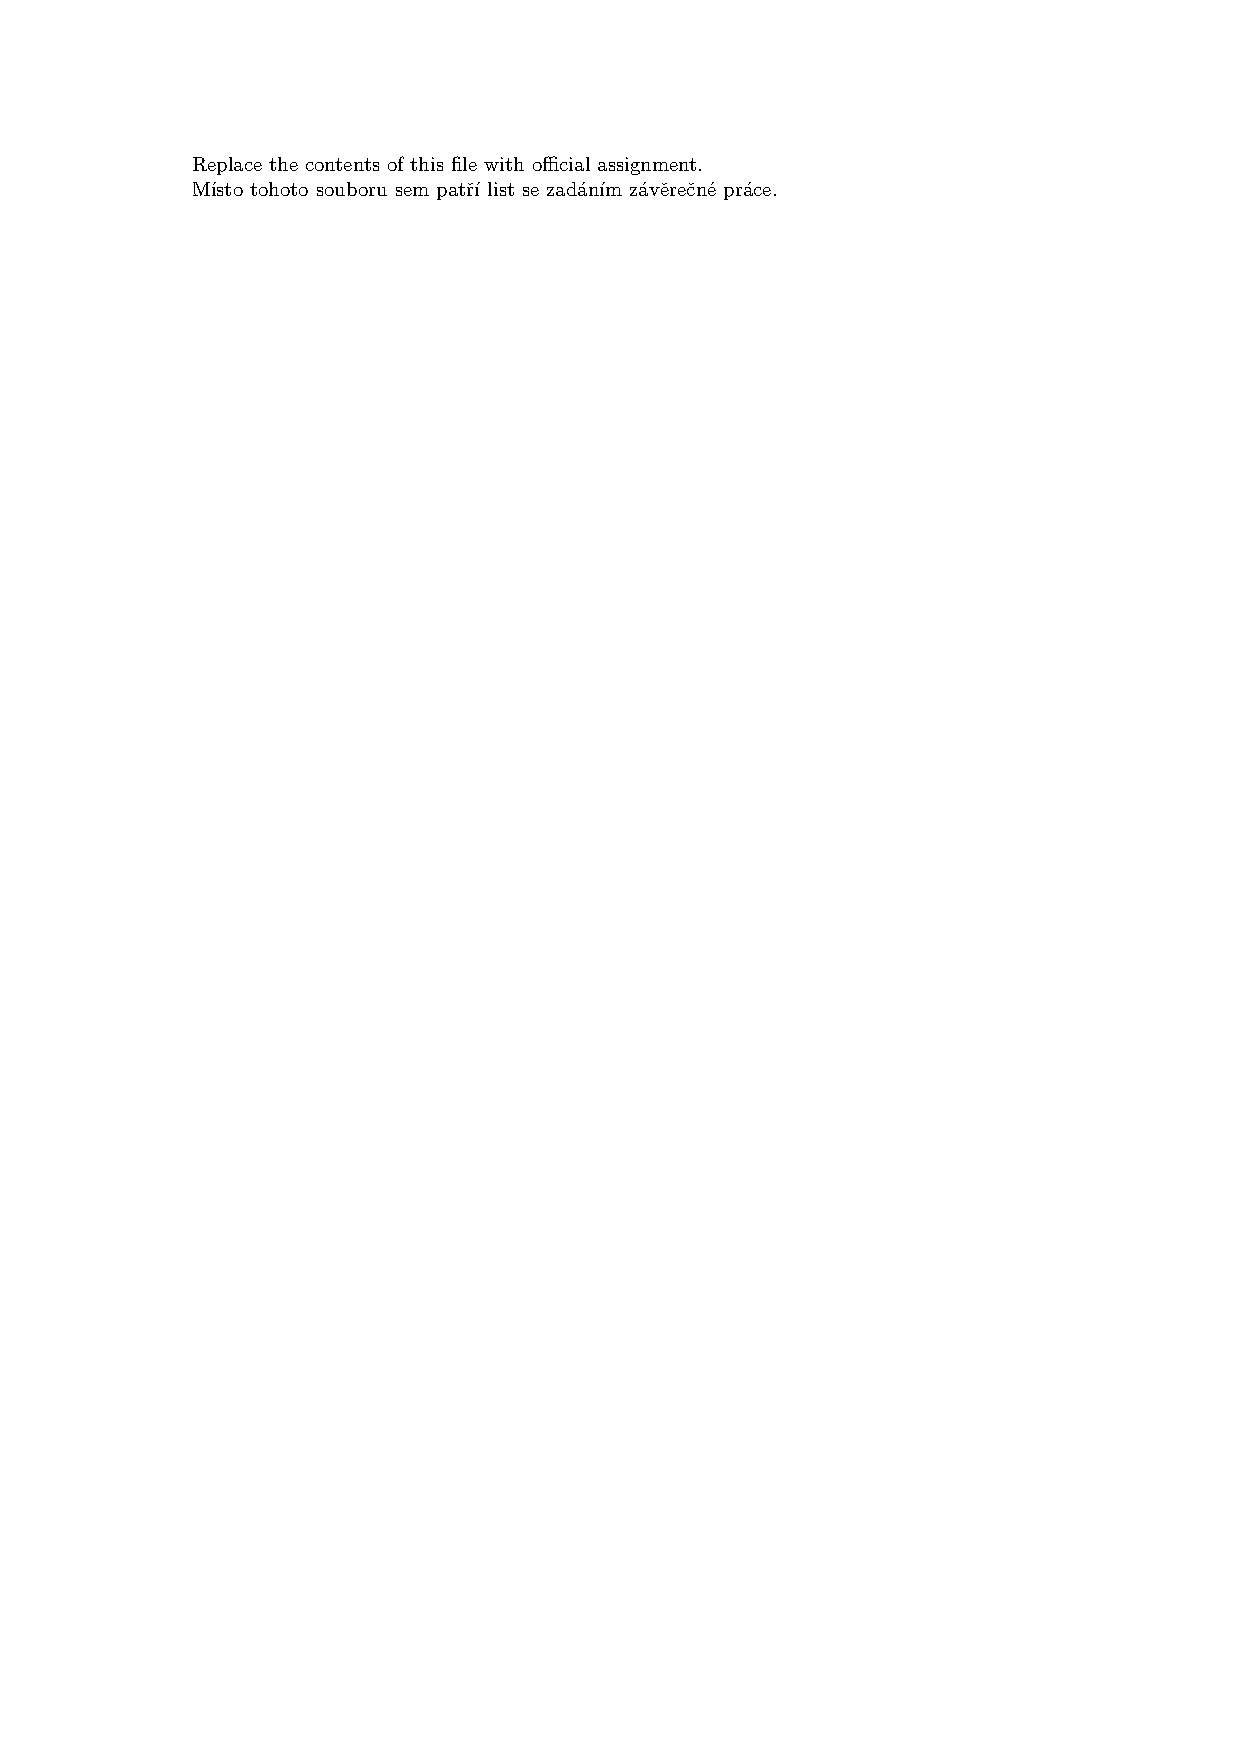
\includepdf[pages={1-}]{example-assignment-include.pdf} % replace this file with your thesis assignment generated from ProjectsFIT

\imprintpage % do not remove this command
\stopTOCentries
%%%%%%%%%%%%%%%%%%%%%%
% list of other contents END
%%%%%%%%%%%%%%%%%%%%%%

%%%%%%%%%%%%%%%%%%%
% ACKNOWLEDGMENT
% FILL IN / MODIFY
% This is a place to thank people for helping you. It is common to thank your supervisor.
%%%%%%%%%%%%%%%%%%%
\begin{acknowledgmentpage}
	Last but not least, I wanna thank me
    
I wanna thank me for believing in me

I wanna thank me for doing all this hard work

I wanna thank me for having no days off

I wanna thank me for, for never quitting

I wanna thank me for always being a giver

And tryna give more than I recieve

I wanna thank me for tryna do more right than wrong

I wanna thank me for just being me at all times

\end{acknowledgmentpage} 
%%%%%%%%%%%%%%%%%%%
% ACKNOWLEDGMENT END
%%%%%%%%%%%%%%%%%%%


%%%%%%%%%%%%%%%%%%%
% DECLARATION
% FILL IN / MODIFY
%%%%%%%%%%%%%%%%%%%
% INSTRUCTIONS
% ENG: choose one of approved texts of the declaration. DO NOT CREATE YOUR OWN. Find the approved texts at https://courses.fit.cvut.cz/SFE/download/index.html#_documents (document Declaration for FT in English)
% CZE/SLO: Vyberte jedno z fakultou schvalenych prohlaseni. NEVKLADEJTE VLASTNI TEXT. Schvalena prohlaseni najdete zde: https://courses.fit.cvut.cz/SZZ/dokumenty/index.html#_dokumenty (prohlášení do ZP)
\begin{declarationpage}
FILL IN ACCORDING TO THE INSTRUCTIONS. VYPLŇTE V SOULADU S POKYNY. Lorem ipsum dolor sit amet, consectetuer adipiscing elit. Curabitur sagittis hendrerit ante. Class aptent taciti sociosqu ad litora torquent per conubia nostra, per inceptos hymenaeos. Cras pede libero, dapibus nec, pretium sit amet, tempor quis. Sed vel lectus. Donec odio tempus molestie, porttitor ut, iaculis quis, sem. Suspendisse sagittis ultrices augue. Donec ipsum massa, ullamcorper in, auctor et, scelerisque sed, est. In sem justo, commodo ut, suscipit at, pharetra vitae, orci. Pellentesque pretium lectus id turpis.

Lorem ipsum dolor sit amet, consectetuer adipiscing elit. Curabitur sagittis hendrerit ante. Class aptent taciti sociosqu ad litora torquent per conubia nostra, per inceptos hymenaeos. Cras pede libero, dapibus nec, pretium sit amet, tempor quis. Sed vel lectus. Donec odio tempus molestie, porttitor ut, iaculis quis, sem. Suspendisse sagittis ultrices augue. Donec ipsum massa, ullamcorper in, auctor et, scelerisque sed, est. In sem justo, commodo ut, suscipit at, pharetra vitae, orci. Pellentesque pretium lectus id turpis.
\end{declarationpage}
%%%%%%%%%%%%%%%%%%%
% DECLARATION END
%%%%%%%%%%%%%%%%%%%

\printabstractpage % do not remove this command

%%%%%%%%%%%%%%%%%%%
% SUMMARY
% FILL IN / MODIFY
% OR REMOVE ENTIRELY (upon agreement with your supervisor)
% (appropriate to remove in most theses)
%%%%%%%%%%%%%%%%%%%
% \begin{summarypage}
% \section*{Summary section}
% 
% \lipsum[1][1-8]
% 
% \section*{Summary section}
% 
% \lipsum[2][1-6]
% 
% \section*{Summary section}
% 
% \lipsum[3]
% 
% \section*{Summary section}
% 
% \lipsum[2]
% 
% \section*{Summary section}
% 
% \lipsum[1][1-8] Lorem lorem lorem.
% \end{summarypage}
%%%%%%%%%%%%%%%%%%%
% SUMMARY END
%%%%%%%%%%%%%%%%%%%

\tableofcontents % do not remove this command
%%%%%%%%%%%%%%%%%%%%%%
% list of other contents: figures, tables, code listings, algorithms, etc.
% add/remove commands accordingly
%%%%%%%%%%%%%%%%%%%%%%
\listoffigures % list of figures
\begingroup
\let\clearpage\relax
\listoftables % list of tables. Remove if you do not have any.
\thectufitlistingscommand % list of code listings. Remove if you do not have any.
\endgroup

%%%%%%%%%%%%%%%%%%%
% ABBREVIATIONS
% FILL IN / MODIFY
% OR REMOVE ENTIRELY
% List the abbreviations in lexicography order.
%%%%%%%%%%%%%%%%%%%
\chapter{\thectufitabbreviationlabel}
	
\begin{tabular}{rl}
LLM & Large Language Model\\
\end{tabular}
%%%%%%%%%%%%%%%%%%%
% ABBREVIATIONS END
%%%%%%%%%%%%%%%%%%%
\resumeTOCentries
\mainmatter\mainmatterinit % do not remove these two commands
%%%%%%%%%%%%%%%%%%%
% THE THESIS
% MODIFY ANYTHING BELOW THIS LINE
%%%%%%%%%%%%%%%%%%%

% Do not forget to include Introduction
%---------------------------------------------------------------
\chapter{Introduction}
% uncomment the following line to create an unnumbered chapter
%\chapter*{Introduction}\addcontentsline{toc}{chapter}{Introduction}\markboth{Introduction}{Introduction}
%---------------------------------------------------------------
\setcounter{page}{1}

\begin{chapterabstract}
% put abstract here %
\end{chapterabstract}

Mutation testing is a technique that involves deliberately introducing artificial errors into a software program to evaluate and improve the performance of a test suite. These modified versions of the program, known as \textit{mutants}, are generated by making slight, intentional changes to the original code. This approach not only assesses the robustness of existing test cases but also supports a variety of software quality assurance processes, such as prioritizing test cases, identifying bugs, and pinpointing fault locations. Mutation testing has evolved to become a high-performing method within contemporary testing and debugging practices.

R\cite{R-base} is an open-source programming language and environment primarily used for statistical analysis, data visualization, and computational research. Initially developed in the early 1990s by Ross Ihaka and Robert Gentleman, R has evolved into one of the most prominent languages in academia, data science, and bioinformatics. Its extensive ecosystem includes powerful packages for statistical modeling, machine learning, and graphical representation of data, making it highly favored by researchers and analysts who require advanced statistical capabilities alongside ease of visualization and reproducibility.

Several mutation testing frameworks have been developed specifically for R, providing tools to evaluate the quality of unit tests by introducing intentional faults (mutations) into the source code and checking if the test suite detects them.

One of the notable mutation testing frameworks for R is mutatr, which integrates directly with testthat\cite{wickham2011testthat}, the most commonly used testing framework for R projects. Mutatr\cite{wickham_mutatr}
 generates mutations by systematically altering R code elements like conditional operators, mathematical operations, and function calls. Despite its seamless integration, mutatr has some limitations, such as limited configurability and flexibility. It can become computationally expensive for larger projects, as it does not efficiently manage mutation selection or parallel execution, thus slowing down the development feedback loop.

This paper presents the development and evaluation of a mutation testing tool for the R programming language. By introducing small, controlled changes into R code, the tool assesses the effectiveness of test suites in detecting faults. The study outlines the tool’s implementation and demonstrates its potential to improve the reliability of R-based software.

%---------------------------------------------------------------
\chapter{Background}
%---------------------------------------------------------------

\begin{chapterabstract}
% put abstract here %
\end{chapterabstract}

\section{Mutation Testing}

Mutation testing is a technique for evaluating the effectiveness of software test suites by systematically introducing small syntactic modifications—known as mutants—into a program \cite{jia2011analysis}. These mutants are created via a process called mutagenesis, whereby specific mutation operators transform the original code to produce slightly altered versions \cite{offutt1996practical}. The fundamental premise is that an effective test suite should be capable of identifying and \textit{killing} these mutants—causing at least one test to fail when executed against a mutant. If no test fails, the mutant remains \textit{alive}, suggesting potential weaknesses in the test suite. This approach provides a more rigorous assessment of test robustness than traditional code coverage metrics, which merely indicate whether parts of the code have been executed \cite{petrovic2018industrial}.

In mutation testing, a mutant refers to a slightly modified version of a software program. These modifications intentionally mimic common faults or errors programmers might make, such as replacing an arithmetic operator (e.g., changing \texttt{+} to \texttt{-}) or altering variable names \cite{jia2011analysis}. The purpose of creating mutants is to test the effectiveness of a software test suite. If a test case fails when executed against a mutant, that mutant is considered \textit{killed}. 

Mutants are generated using predefined mutation operators, which define the specific rules or types of changes applied to the original code to produce mutants \cite{offutt1996practical}. These operators simulate typical programming mistakes or variations to strengthen test suites. For example, a mutation operator might systematically replace relational operators (\texttt{>} with \texttt{<}) or insert exceptions such as division by zero \cite{jia2011analysis}. Through these operators, developers can create diverse mutants, enhancing the robustness and completeness of their testing strategies.

The effectiveness of a test suite is quantified using a metric known as the mutation score, defined as the proportion of killed mutants relative to the total number of generated mutants \cite{jia2011analysis}. A higher mutation score indicates a more fault-sensitive and robust test suite. However, practical application of mutation testing, especially in large-scale software systems, presents significant computational challenges \cite{petrovic2018industrial}. The necessity to execute the full test suite against each mutant results in substantial computational overhead, particularly in complex packages containing numerous tests. Additionally, the existence of equivalent mutants, which behave identically to the original program despite syntactic changes, complicates mutation testing. These equivalent mutants cannot be killed by any test, potentially deflating the mutation score if not identified correctly \cite{offutt1996practical}.

The conventional procedure of mutation analysis is depicted in Figure~\ref{fig:MutationAnalysis}. A set of faulty program versions—mutants, denoted as \( p' \)—is systematically derived from the original program \( p \) through small syntactic modifications guided by predefined mutation operators. For instance, as shown in Table~\ref{tab:MutationOperation}, a mutant \( p' \) can be created by altering a logical AND operator (\texttt{\&\&}) to a logical OR operator (\texttt{||}). This intentional alteration results in behaviorally distinct program versions, which are subsequently tested to evaluate the effectiveness of the existing test suite \cite{jia2011analysis}.

%!!!Introduce equivalent mutants!!!%

\section{R language}

R is a widely-used open-source programming language designed primarily for statistical computing, data analysis, and graphical visualization \cite{rcore2024}. Due to its extensive package ecosystem and versatility, R has become one of the leading tools for exploratory data analysis, predictive modeling, and reproducible research \cite{wickham2014advanced}. Its rich syntax enables users to express complex analytical workflows concisely, facilitating rapid prototyping and iterative development \cite{wickham2019r4ds}.

R fosters a strong community-driven environment, supported by repositories such as CRAN (Comprehensive R Archive Network) and Bioconductor, which collectively offer thousands of libraries covering diverse domains within data science and statistics \cite{gentleman2004bioconductor}. Its interactive development environment facilitates experimentation and collaboration, enabling researchers to seamlessly share methods, results, and visualizations \cite{wickham2019r4ds}.

\texttt{testthat} is an R library specifically designed to simplify and encourage automated software testing practices \cite{wickham2011testthat}. Developed by Hadley Wickham, it has become the most widely used testing framework within the R community. \texttt{testthat} provides a straightforward and expressive syntax, allowing developers to clearly articulate test expectations and quickly verify the correctness of their functions. By supporting unit testing and test-driven development, it enhances software reliability and encourages developers to rigorously consider the behavior of their code \cite{wickham2015rpackages}.

The library integrates seamlessly into the standard R package development workflow, facilitating continuous integration, debugging, and reproducible test suites \cite{wickham2015rpackages}. With \texttt{testthat}, developers can efficiently manage complex test scenarios through simple test expressions, making it ideal for both beginners and advanced users who aim to ensure high-quality and robust R code.

%introduce R package structure%


\section{Importance}

Mutation testing is recognized as one of the most powerful techniques to evaluate the effectiveness and reliability of test suites in software development. It involves intentionally introducing faults, known as mutants, into a program's source code and determining if the existing tests can detect these faults. If tests fail to detect these mutants, it indicates weaknesses in the test suite, highlighting areas that require improvement.

The industrial importance of mutation testing has been demonstrated notably by Petrovic and Ivankovic in their comprehensive case study conducted at Google \cite{petrovic2018industrial}. Their research evaluated mutation testing on an industrial scale, involving over 30,000 developers and 1.9 million change sets across multiple programming languages. They concluded that mutation testing significantly enhances test suite quality by systematically identifying test coverage deficiencies, although it also poses challenges due to its computational complexity and resource demands. The findings emphasize the practicality and benefit of integrating mutation testing into large-scale, real-world software engineering processes.

\begin{figure}[!htbp]
    \centering
    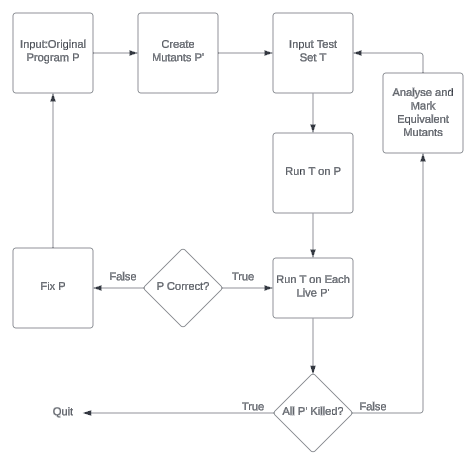
\includegraphics[width=\linewidth]{images/MutationProcess.png}
    \caption{Generic process of mutation analysis.~\cite{offutt2010mutation}}
    \label{fig:MutationAnalysis}
\end{figure}

\begin{figure}[!htbp]
    \centering
    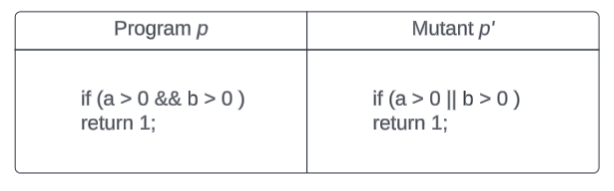
\includegraphics[width=\linewidth]{images/MutationOperation.png}
    \caption{An Example of Mutation Operation ~\cite{offutt2010mutation}.}
    \label{fig:MutationOperation}
\end{figure}

%---------------------------------------------------------------
\chapter{Solution}
%---------------------------------------------------------------

\begin{chapterabstract}
% put abstract here %
\end{chapterabstract}

\section{Design constraint}

\section{Application data flow}

%Data flow diagram showing where the data is coming from and where going %

\section{Technologies}

\subsection{GoogleTest}
%put google test here%

\subsection{Library rcpp11}
%put rcpp11 here%

\subsection{Library furrr}

\subsection{Library testthat}

\section{Implementation Decisions}

\subsection{Mutator class}

%put some pseudocode here%

\subsection{ASTHandler class}

%put some pseudocode here%

\subsection{mutateR class}

%put some pseudocode here%

\subsection{Operators hierarchy}

%put some pseudocode here, maybe a class diagram%


%---------------------------------------------------------------
\chapter{Optimization}
%---------------------------------------------------------------

\begin{chapterabstract}
% put abstract here %
\end{chapterabstract}

\section{Background}

\subsection{LLMs used}

\section{Equivalent Mutants}

\subsection{Detection techniques}

\subsection{Prompt creation}

%cite the Chinese paper%

%---------------------------------------------------------------
\chapter{Evaluation}
%---------------------------------------------------------------

\begin{chapterabstract}
% put abstract here %
\end{chapterabstract}

\section{Test runs on various size packages}


\subsection{Small packages}

%run on itself%

\subsection{Medium packages}

%gtable?%

\subsection{Big pacakges}

%dplyr%

%---------------------------------------------------------------
\chapter{Conclusion}
%---------------------------------------------------------------

\begin{chapterabstract}
% put abstract here %
\end{chapterabstract}


 % include `text.tex' from `text/' subdirectory

\appendix\appendixinit % do not remove these two commands

\chapter{Appendix}
 % include `appendix.tex' from `text/' subdirectory

\backmatter % do not remove this command
\printbibliography % print out the BibLaTeX-generated bibliography list

\chapter{Obsah příloh}
% Contents of the attachment

	\dirtree{%
		.1 /.
		.2 readme.txt\DTcomment{stručný popis obsahu média}.
		.2 exe\DTcomment{adresář se spustitelnou formou implementace}.
		.2 src.
		.3 impl\DTcomment{zdrojové kódy implementace}.
		.3 thesis\DTcomment{zdrojová forma práce ve formátu \LaTeX{}}.
		.2 text\DTcomment{text práce}.
		.3 thesis.pdf\DTcomment{text práce ve formátu PDF}.
	}
 % include `medium.tex' from `text/' subdirectory

\end{document}
